\documentclass{article}
\usepackage{arxiv}
\usepackage[utf8]{inputenc} % allow utf-8 input
\usepackage[T1]{fontenc} % use 8-bit T1 fonts
\usepackage{hyperref} % hyperlinks
\usepackage{url} % simple URL typesetting
\usepackage{booktabs} % professional-quality tables
\usepackage{amsmath}
\usepackage{amssymb}
\usepackage{mathtools}
\usepackage{amsfonts} % blackboard math symbols
\usepackage{nicefrac} % compact symbols for 1/2, etc.
\usepackage{microtype} % microtypography
\usepackage{lipsum}
\usepackage{graphicx}
\usepackage{subcaption}
\graphicspath{ {./images/} }
\title{Extending Neural Collaborative Filtering with Outer Product and Residual Networks}

\author{
Shriram Varadarajan \\
Department of Electrical and Computer engineering\\
University of Iowa\\
Iowa City, IA, 52242 \\
\texttt{shriram-varadarajan@uiowa.edu} \\
\And
Jacob Nishimura \\
Department of Electrical and Computer engineering\\
University of Iowa\\
Iowa City, IA, 52242 \\
\texttt{jacob-nishimura@uiowa.edu} \\
\And
Joseph Kim \\
Department of Biomedical Engineering\\
University of Iowa\\
Iowa City, IA, 52242 \\
\texttt{joseph-kim-3@uiowa.edu} \\
}


\begin{document}
\maketitle

\begin{abstract}
State of the art embedding-based recommendation models have been proposed that use learned similarities (e.g. Multilayer Perceptron-based methods) instead of more traditional, dot product-based methods. A further framework was proposed that employs an outer product of the user and item embeddings to generate a 2-dimensional interaction map which can then be processed using Convolutional Neural Networks to generate predictions. In this work, the authors implement examples of both types of framework and also extend the outer product framework by processing the interaction map with a Residual Network. Experiments on two MovieLens datasets compare the performance of all models and demonstrate both the power of well-trained dot product recommender systems and opportunities for future research.
\end{abstract}

\keywords{Collaborative filtering \and Recommender systems \and Content-based filtering}

\section{Introduction}
In the current age of web browsing, recommendations are given in numerous applications ranging from entertainment to shopping to social media. Many systems have far too many items for a user to consistently find compelling content on their own. For example, the iOS app store has millions of apps, Amazon's marketplace has hundreds of millions of items, and YouTube hosts billions of videos. Recommendations are user-personalized suggestions derived from known interests from past experiences or behavior. Recommendation (or recommender) systems are systems which use various algorithms to generate and rank suggestions to show the user. While users can find items using search, recommender systems are able to surface items the user may not have thought of or even known existed. Good recommender systems can yield benefits for both the user and the business: users can be given more relevant and compelling recommendations leading to a better experience, and a better experience can promote more user engagement and growth.

In general, recommender systems are composed of three parts: candidate generation, scoring, and re-ranking. The recommender system takes in a single or numerous queries (information about the user such as an ID number or previous interactions, and other context such as the time of day or the user's device) and outputs a set of items (such as movies, apps, social media posts). The candidate generation stage (which may consist of multiple, separate generators) uses the queries to select a small (relative to the total amount of items in the system) set of items for further processing. The scoring stage takes in the generated candidates, determines a score for each item, and ranks the items according to that score. Finally, the re-ranking stage can consider additional criteria to change the recommendations before being served to the user. Items can be moved or discarded in this stage for business reasons (removing content the user isn't eligible to play, filtering out mature content) or for recommendation quality reasons (freshness, diversity, etc).

Focusing on candidate generation, multiple approaches are used today. Two common approaches are content-based filtering or collaborative filtering. Both approaches utilize embeddings (projections from high-dimensional, categorical information to relatively low-dimensional, continuous vector representations) to determine similarity between entities. Content-based filtering finds similar items to those the user has already indicated they like. For example, if a user has shown that they enjoy action novels, the system can find similar action novels to recommend the user. Some advantages to content-based filtering are that it does not need other user’s information to make recommendations and can capture the specific interests of the user. A large downside to content-based filtering is that it can require a lot of domain knowledge to extract relevant features. Content-based filtering typically uses explicit feedback, such as numeric ratings the user gives to novels they've read.

Unlike content-based filtering, collaborative filtering uses interest data from other users to power its recommendations. Collaborative filtering is built off the assumptions that users with similar interactions share some number of preferences, and users that have shared preferences may respond similarly to the same items. For example, given users A and B have both bought some of the same items in the past, a new item that user A buys may also interest user B. Collaborative filtering has the advantage of not requiring large amounts of domain knowledge, as the system is able to learn effective embeddings for the data by itself. It is also able to recommend the user new items that are separate from the user's current known interests (serendipity). A major downside to collaborative filtering is that collaborative filtering cannot handle new items that the system has come up with since it is difficult to create embeddings for items that the model hasn’t seen yet. Unlike content-based filtering, collaborative filtering can often also use implicit feedback, such as assuming the user is interested in each item they've bought. While this can have drawbacks, such as aiding "clickbait" content, it also generally allows much greater amounts of data to be used for learning.

Traditionally, collaborative filtering uses Matrix Factorization (MF) to learn and utilize an embedding model. Using user-item interactions as inputs to a Matrix Factorization model allows the model to learn embeddings for the users and items. The model can then be used for new user-item pairs by calculating the dot product between the user's embedding and the item's embedding: $\hat{y}_{ui} = f(u,i|p_u,q_i) = \textbf{p}^T_u\textbf{q}_i = \sum{p_{uk}q_{ik}}$, where $\hat{y}_{ui}$ is the interaction and $\textbf{p}_u$ and $\textbf{q}_i$ are the embedding vectors for user \textit{u} and item \textit{i}.

He et al. proposed Neural Collaborative Filtering (NCF) as a new framework for collaborative filtering which combined traditional MF with a multilayer perceptron to improve recommendation performance compared to previous MF-based techniques (element-wise Alternating Least Squares, Bayesian Personalized Ranking) \cite{he2017neural}. The original NCF paper used a multilayer perceptron to model additional non-linearities in user-item interactions. Further, He et al. proposed Outer Product-based Neural Collaborative filtering, a technique which applied the outer product operation to user and item embeddings generating a 2-dimensional interaction map \cite{he2018outer}. The approach could then use Convolutional Neural Network models on the interaction map to extract features and finally predict the interaction. In both cases, the frameworks encouraged further experimentation with network architecture and parameters to improve performance.

In this manuscript, the authors proposed applying recent advances in neural network training (batch normalization, dropout) and architecture to the inner and outer product NCF frameworks.

\section{Problem Definition}
\label{sec:Problem Definition}
To test the effectiveness of modifications to the NCF and outer-product frameworks, changes were applied to the problem of generating movie recommendations based on implicit feedback. Given $M$ users, $N$ items, and an $M$x$N$ user-item matrix, $\mathbf{Y}$, $y_{ui} = 1$ if user $u$ had interacted with item $i$, otherwise $y_{ui} = 0$. He et al. pointed out that this could pose challenges as a value of 1 does not necessarily mean the user liked an item, and a value of 0 does not mean the user disliked an item (they could just be unaware of the item) \cite{he2017neural}. The recommendation problem was then given as the problem of estimating scores for unobserved user-item pairs in $\mathbf{Y}$.

The deep neural networks to be compared were built using TensorFlow with Keras and took in a pair consisting of user ID and movie ID. The networks then output a probability that the user would interact with the movie. To evaluate the performance of the models, the authors used two metrics: Hit Ratio (HR) and Normalized Discounted Cumulative Gain (NDCG). To calculate these metrics, the models were fed in 99 items that the user had not previously interacted with and one test item that the user had interacted with before. Hit Ratio measured whether the test item appeared in the top-N of the 100 ranked items. Normalized Discounted Cumulative Gain measured how-highly the item was ranked within the top-N.

The traditional Neural Collaborative Filtering (NCF) model took the user and item embeddings, applied Matrix Factorization and a neural network to the embeddings, and had a final block of layers to compute the probability. The outer-product Neural Collaborative Filtering model also took the user and item embeddings. This model computed the outer product between the two embeddings, resulting in a 2-dimensional, $D$x$D$ matrix known as the interaction map. The CNN architecture, ResNet, was applied to the interaction map to extract features, and a final block of layers again computed the probability.

\textbf{Inputs}: The input to our models were pairs of user ID and movie ID converted into Dense vectors using embeddings. Each Dense embedded vector had $d$ dimensions, where d was an adjustable parameter for the size of the embedding.

\textbf{Outputs}: The output of our models was a probability between 0 and 1. The probability represented the likelihood that a user $u$ would interact with an item $i$.

\section{Data}
\label{sec:Data}

\begin{itemize}
\item Available data included user-given movie ratings, user-applied movie tags, and two additional files containing links to each movie's IMDB and TMDB. The movie ratings contained unique identifiers for the user and the movie, a rating score, and the time the rating was made. The movies also had associated genres and titles. Data that was not available included users' text reviews for further word processing and text similarity.
\item The movies were collected from the website \url{https://www.themoviedb.org/} by the GroupLens research group at the University of Minnesota Twin Cities. This database hosted information on millions of movies, TV shows, and actors. The site was originally conceived as a donation from the Online Media Database, which is an online collaborative database intended to share content published under a Creative Commons license. The data was created by 162,541 users between January 09, 1995 and November 21, 2019. This dataset was generated on November 21, 2019.
\item MovieLens datasets were generally distributed in the CSV format. The authors used the built-in CSV parser in the pandas library to extract the data. GroupLens distributed a multitude of datasets for various uses (education, research, performance testing). The authors proposed using the Latest Small dataset for initial development and training, then switching to the stable 1M dataset for performance comparisons. The small dataset was formatted with 100,836 ratings, 3683 tags, 9,742 movies, and 610 users collected between March 1996 and September 2018. The stable 1M dataset had 1 million ratings from 6000 users on 4000 movies.

\end{itemize}


\subsection{Tables}

\begin{table}[h]
\caption{Ratings}
\centering
\begin{tabular}{llll}
\toprule
userId & movieId & Rating & Timestamp \\
\midrule
1 & 1 & 4 & 964982703 \\
1 & 3 & 4 & 964981247 \\
1 & 6 & 4 & 964982224 \\
\bottomrule
\end{tabular}
\label{tab:table1}
\end{table}

\begin{table} [h]
\caption{Tags}
\centering
\begin{tabular}{llll}
\toprule
userId & movieId & Tag & Timestamp \\
\midrule
2 & 60756 & funny & 1445714994 \\
2 & 60756 & Highly quotable & 1445714996 \\
2 & 60756 & will ferrell & 1445714992 \\
\bottomrule
\end{tabular}
\label{tab:table2}
\end{table}

\begin{table}[h]
\caption{MovieLens}
\centering
\begin{tabular}{llll}
\toprule
Users & Movies & Ratings \\
\midrule
6040 & 3076 & 1000203 \\
\bottomrule
\end{tabular}
\end{table}

\section{Methods}
\subsection{Data Preparation and Training}
As shown in Section 3.1 Table 1, the MovieLens datasets contain explicit feedback in the form of ratings. As discussed in Section 2, each rating is assumed to be a positive data point in the conversion to implicit feedback. In order to have negative data points to train against, four movies are sampled at random for each user from the set of movies the user has not rated. New training samples are generated at the same 4:1 ratio for each training epoch.

He et al. demonstrate that recommendation with implicit feedback can be treated as a binary classification task \cite{he2017neural}. That is, predicting that a user will either have or have not interacted with a given movie. Viewing the problem from this perspective leads to the use of binary cross-entropy loss for the optimization problem.

For testing purposes, each user's most recent rating is used as a testing entity. This helps avoid look-ahead bias in the training and evaluation process. To fill out the evaluation data, 99 negative interactions are sampled for each user.

\subsection{Evaluation Metrics}
To compare model performance, two main metrics are used: Hit Ratio (HR) and Normalized Discounted Cumulative Gain (NDCG). The models are used to generate interaction probabilities for the 100-item set consisting of the one test interaction and the 99 negative interactions. The interactions are ranked by their probability, and (like the original NCF paper) the list of the top 10 items is used for both metrics (notated as HR@10 and NDCG@10). The Hit Ratio (for each user $u$ with target item $i$) is defined below, and averaging out the hit ratio over all users in the test set yields the overall hit ratio (percentage of users whose test entity was in their top 10 list).

\[
HR@10 = 
\begin{cases}
1 & \text{if $i$ in top 10}, \\
0 & \text{otherwise}
\end{cases}
\]

Similarly, NDCG@10 is defined below for target item $i$ in position $p$ (i.e. the top item is in the 1st position) of the top 10 list. The NDCG@10 can be interpreted as yielding a higher score when the test entity is placed at a higher position in the ranked list. By definition, the highest possible NDCG is achieved when the highest-ranked item is the target item. Like with HR@10, the NDCG@10 values for each user are averaged out to determine the average NDCG@10.

\[
NDCG@10 = 
\begin{cases}
\frac{\ln 2}{\ln(p + 1)}& \text{if $i$ in top 10}, \\
0 & \text{otherwise}
\end{cases}
\]

\subsection{Models}
The first three models covered in this section originate from the original Neural Collaborative Filtering paper \cite{he2017neural}. The fourth model originates from the Outer Product-based Neural Collaborative Filtering paper \cite{he2018outer}. Finally, the fifth model is a novel extension to the Outer Product-based method. All the models tested share the same data input scheme: users and movies are converted into $D$-dimensional embedding vectors: $\mathbf{p}_u$ and $\mathbf{q}_m$ respectively. Each model manipulates these embeddings differently to extract information for predicting whether the user would interact with the movie.

\subsubsection{Generalized Matrix Factorization}
After obtaining the user and movie embedding vectors, the Generalized Matrix Factorization (GMF) model takes the element-wise product between the two vectors. This product vector is then fed through a dense layer to obtain the final prediction. He et. al define this model below, where $a_{out}$ is the activation function and $\mathbf{h}$ is the weight vector of the output layer. In the case where $a_{out}$ is the identity and $\mathbf{h}$ is a vector of 1s, this is equivalent to a traditional Matrix Factorization method \cite{he2017neural}.

\[
\hat{y}_{um}=a_{out}(\mathbf{h}^{T}(\mathbf{p}_u\odot\mathbf{q}_m))
\]

\begin{center}
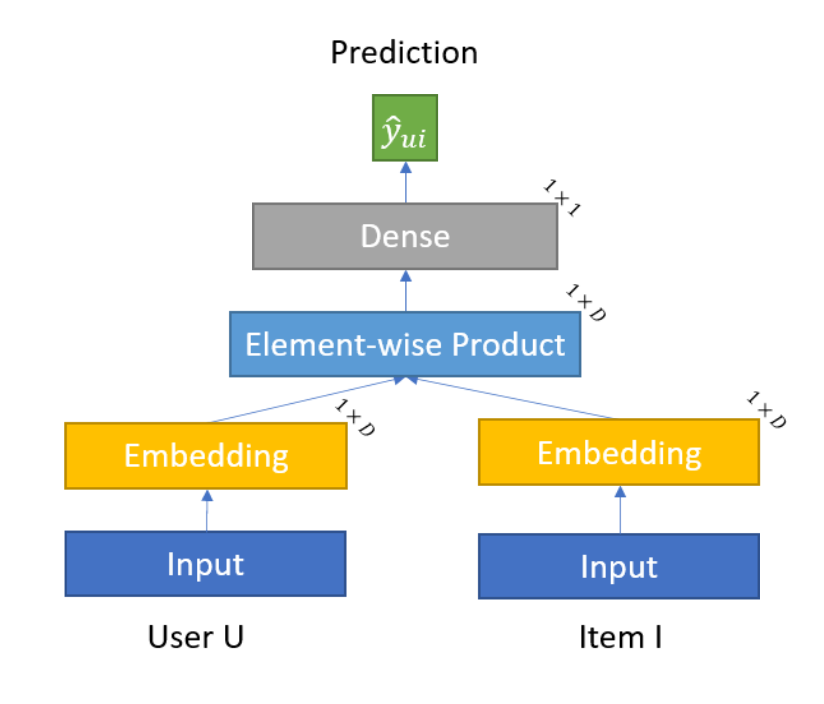
\includegraphics[scale=0.275]{GMF_Diagram}

Block diagram of the General Matrix Factorization model
\end{center}

The final layer uses a sigmoid activation function to match the original GMF model. After some experimentation, the final GMF models were trained using the Adam optimizer with a learning rate of 0.01. 

\subsubsection{Multilayer Perceptron}
Rather than taking the element-wise product of the embedding vectors, the Multilayer Perceptron (MLP) model concatenates them together then passes the concatenated vector through multiple fully-connected layers. Using multiple fully connected layers allows the model to learn more non-linear interactions between the user and movie embeddings. Using $X^\frown Y$ as vector concatenation and given $\mathbf{W}_n$, $\mathbf{b}_n$, and $a_{n}$ as the weights, biases, and activation function for the nth layer, the n-layer MLP model can be expressed mathematically as:

\begin{align*}
\mathbf{x}_{in} &= \mathbf{p}_u\frown \mathbf{q}_m \\
\mathbf{x}_{1} &= a_{1}(\mathbf{W}^T_{1}\mathbf{x}_{in} + \mathbf{b}_{1})\\
&...\\
\mathbf{x}_{n-1} &= a_{n-1}(\mathbf{W}^T_{n-1}\mathbf{x}_{n-2} + \mathbf{b}_{n-1})\\
\hat{y}_{ui} &= a_{out}(\mathbf{W}^T_{n}x_{n-1} + \mathbf{b}_{n})
\end{align*}

\begin{center}
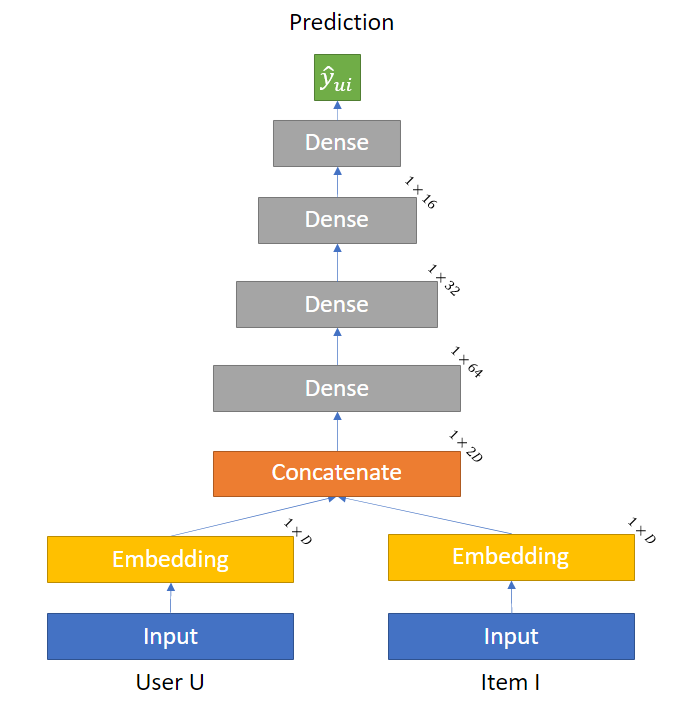
\includegraphics[scale=0.4]{MLP_Diagram}

Block diagram of the Multilayer Perceptron model
\end{center}

Like the GMF model, the MLP model also uses a sigmoid activation function on the final layer. The GMF models were trained using the Adam optimizer with a learning rate of 0.001.

\subsubsection{Neural Matrix Factorization}
The Neural Matrix Factorization (NeuMF) model is similar to an ensemble of the GMF and MLP models. In this paper's implementation, the user and movie embeddings are passed into GMF and MLP models yielding predictions $\hat{y}_{GMF}$ and $\hat{y}_{MLP}$. The final output of this implementation of the NeuMF model is the weighted sum of these two intermediate outputs:

\[
\hat{y}_{ui} = \alpha\hat{y}_{GMF} + (1 - \alpha)\hat{y}_{MLP}
\]

The NeuMF model sets $\alpha$ as trainable to determine an optimal weighting for each model to contribute.

\begin{center}
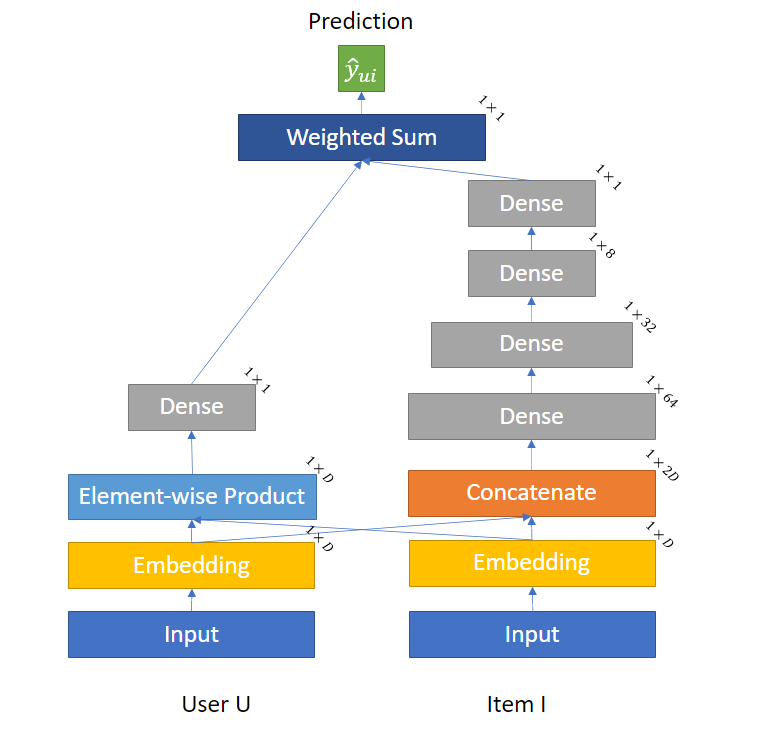
\includegraphics[scale=0.4]{NeuMF_Diagram}

Block diagram of the Neural Matrix Factorization model
\end{center}

The NeuMF models were trained using the Adam optimizer with a learning rate of 0.01.

\subsubsection{Outer Product-based Neural Collaborative Filtering}
The Outer Product model is designed based on the framework designed by He et al. in \cite{he2018outer}. The idea was to design a recommender system using the same NCF methods while introducing an outer product to create an interaction map. As previously mentioned, this representation resulted in a 2-dimensional, $D$x$D$ matrix known as the interaction map, where D refers to the embedding size. Notably, the interaction map's diagonal entries are the element-wise product of $\mathbf{p}_{u}$ and $\mathbf{q}_{m}$. The interaction map's non-diagonal entries are able to more explicitly represent interactions between different dimensions of the embeddings. The interaction map can be defined as:

\[
\mathbf{M} = \mathbf{p}_{u} \odot \mathbf{q}_{m}
\]

As such, individual entries in the map are:

\[
\mathbf{M}_{ij} = \mathbf{p}_{ui}\times\mathbf{q}_{mj}
\]

The interaction map was fed into a network consisting of two convolution layers with ReLU activation, a pooling layer, and a Dense layer with sigmoid activation to generate a final recommendation. 

\begin{center}
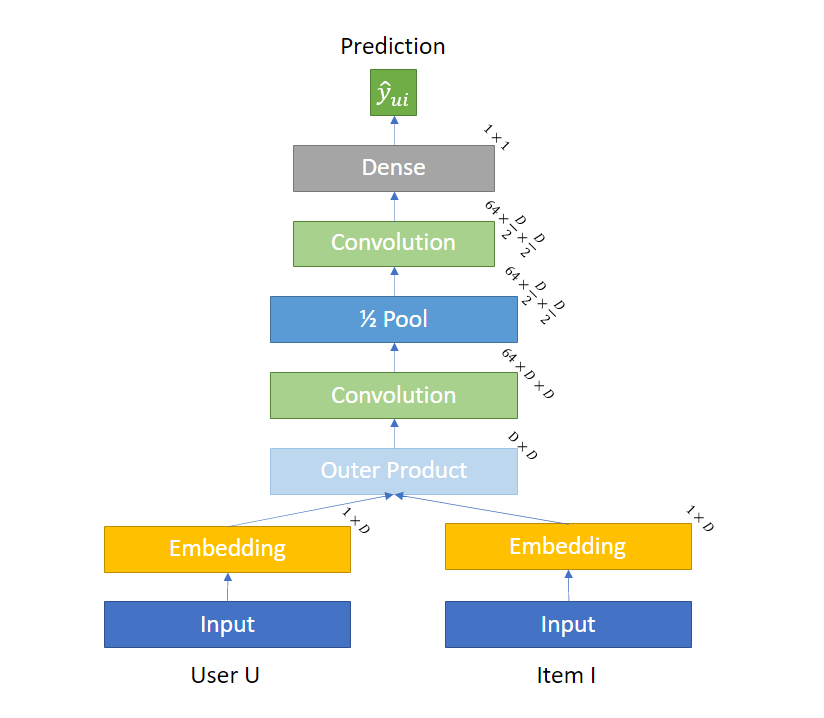
\includegraphics[scale=0.4]{OuterProduct_Diagram}

Block diagram of the Outer Product model
\end{center}

The Outer Product models were trained using the Adam optimizer with a learning rate of 0.001.

\subsubsection{Outer Product-based Residual Network}
Like the original Outer Product model, the ResNet model learned embeddings for users and items then took the outer product of those embeddings to generate an interaction map. The ResNet model then employs residual blocks and residual downsampling blocks to extract information from the interaction map. The residual blocks employ shortcut connections which allow the blocks to learn a residual function instead of the original function (i.e. learn $f(x) = H(\mathbf{x}) - \mathbf{x}$ instead of $H(\mathbf{x})$). He et al. hypothesize these residual functions may be easier to learn \cite{he2015deep}. This allows the ResNet model to be much deeper than the original outer product model while still being feasibly trainable. The final ResNet model has 20 convolutional layers (along with ReLU activations, batch normalization, and the shortcut connections) which balanced performance with training speed, allowing the authors to iterate on the model more quickly.

\begin{center}
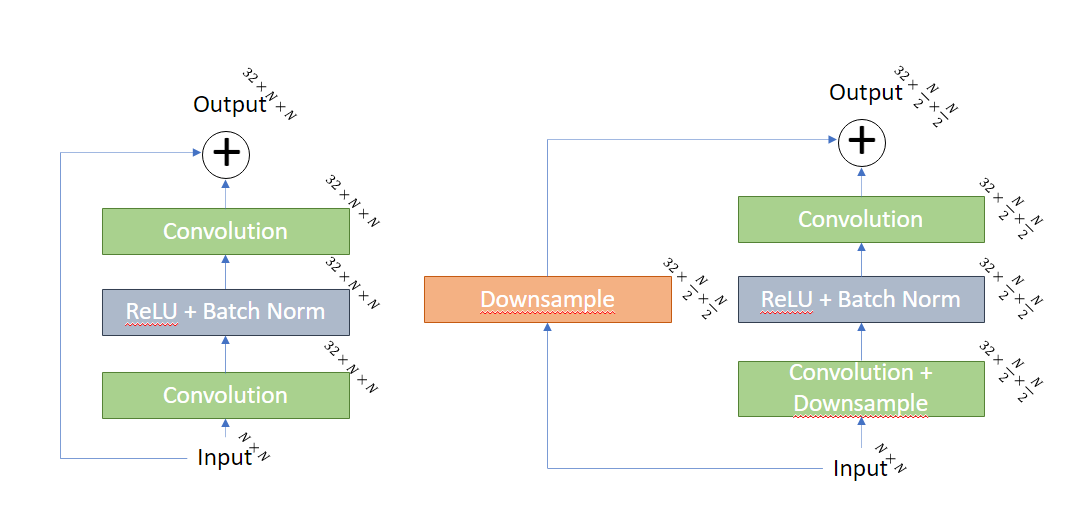
\includegraphics[scale=0.4]{ResBlocks_Diagram}

Residual block (left) and Downsampling Residual block (right)
\end{center}

The residual blocks were chosen to use 32 filters per convolutional layer to balance learning ability with training time and computational complexity.

\begin{center}
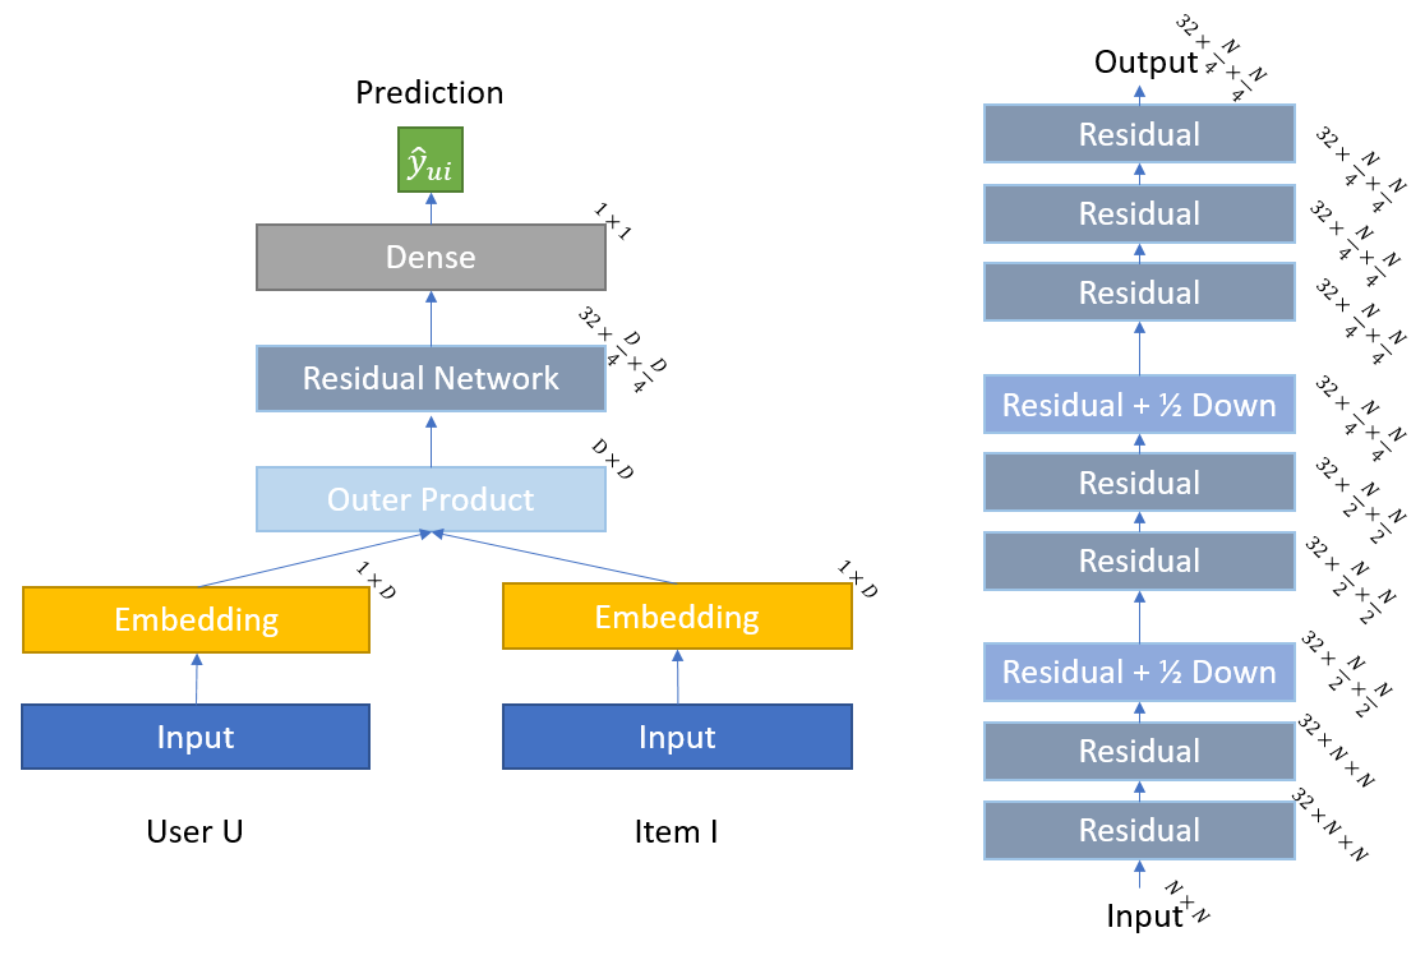
\includegraphics[scale=0.4]{ResNet_Diagram}

Complete ResNet Model (left) and Residual Network (right)
\end{center}

The ResNet models were trained using the Adam optimizer with a learning rate of 0.005.

\section{Experiments and Results}
\subsection{Overall Performance}
After developing the models using the 100k MovieLens dataset, the models were trained and evaluated on the 1 Million Movie Lens dataset. Hit Ratio, NDCG, and loss values were collected for an untrained model (Epoch 0) and over the course of 10 training epochs for all models discussed in the Methods section. Additionally, these values were collected for the best-performing versions of each of the architectures. 

\begin{center}
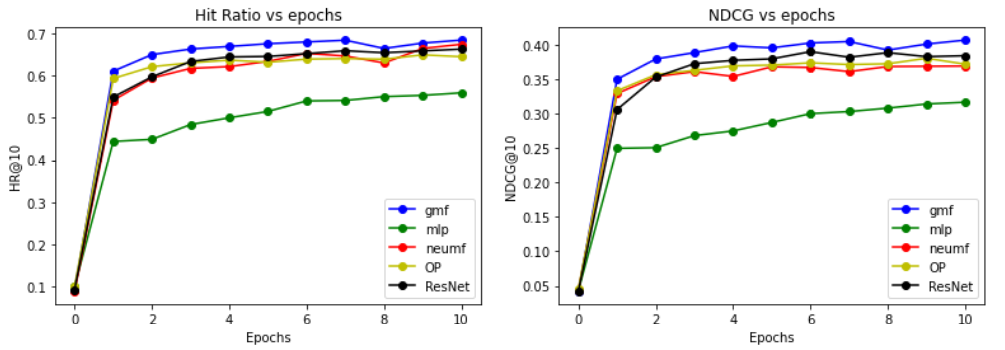
\includegraphics[scale=0.6]{HR_NDCGs}

HR@10 over 10 epochs (left) and NDCG@10 over 10 epochs (right) for models with embedding dimension = 8
\end{center}

\begin{center}
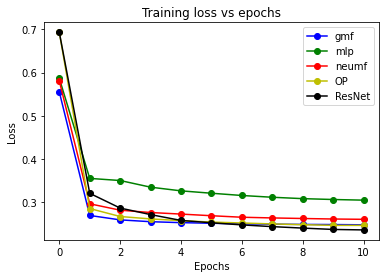
\includegraphics[scale=0.5]{loss}

Training loss over 10 epochs for models with embedding dimension = 8
\end{center}

After 10 epochs, all the models tested were making marginal improvements on their loss functions. That is, almost all performance gains had been realized. For both Hit Ratio and NDCG, all the models except the MLP performed very similarly. Interestingly, the original Neural Collaborative Filtering paper demonstrated the GMF model underperforming the MLP and NeuMF models consistently through the epoch range tested, whereas the opposite occurs here. One explanation for this difference could be small changes in implementation or hyperparameters such as learning rates or regularization coefficients.

While the Outer Product model performs well, changing the convolutional layers to a ResNet shows consistent improvements. Since the ResNet architecture used was relatively shallow (due to hardware and training time constraints), the authors hypothesize that further performance improvements could be made by adding more residual blocks to the ResNet model.

\subsection{Effect of Embedding Dimensions}
For further testing, the models were created using four different sizes for the embedding vectors: 4, 8, 16, and 32. 

\begin{center}
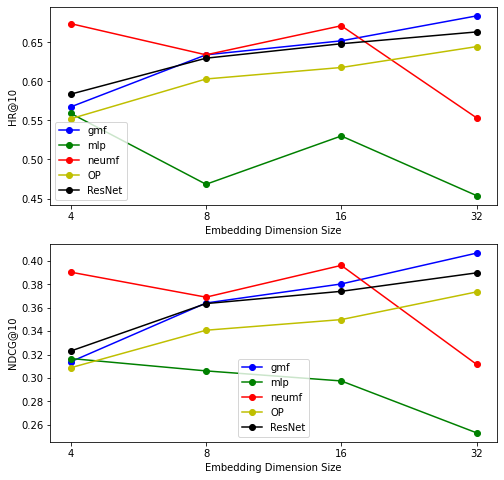
\includegraphics[scale=0.5]{images/Embedding_Size.png}

Hit Ratio and NDCG for the 5 models with varying embedding dimensions
\end{center}

The GMF, Outerproduct, and ResNet models both show positive increases on both metrics with larger embedding dimensions while the MLP and NeuMF models don't show a clear correlation between either metric and embedding size. Again, this departs slightly from the results reported in the original Neural Collaborative Filtering \cite{he2017neural} paper, where the MLP and NeuMF model performances were observed to have a positive correlation with respect to embedding size. Again, one explanation could be implementation or training details. One encouraging result is that NeuMF performance shows similar trends as the MLP and GMF models, showing that it is following an ensemble approach. That is, the NeuMF model performs well on embedding sizes where the GMF and MLP perform well, and it performs less well on embedding sizes where the MLP performs less well. However, the model may not be learning a good weighting parameter $\alpha$ since it seems to overemphasize the MLP component and perform much worse when the MLP performs worse. He et al. propose an approach that may mitigate this: concatenate the GMF and MLP's final (pre-output) layers and then pass that prediction vector through a single output layer \cite{he2017neural}. Improvements may be made in the future by improving the MLP model's performance and experimenting with different ensemble approaches.


\subsection{Dataset Size}
The GMF model was trained and tested on the MovieLens Latest Small dataset to compare performance with the same model trained and tested on the MovieLens 1 Million dataset.

\begin{center}
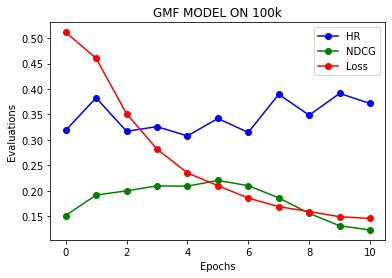
\includegraphics[scale=0.5]{GMF_100k}

Hit Ratio, NDCG, and Loss of the GMF model on the MovieLens Latest Small dataset
\end{center}

While training loss continues to decrease with each epoch, the Hit Ratio oscillates in the same range and NDCG increases then rapidly decreases. Taking a closer look at the two datasets, the Latest Small dataset contains 100,836 ratings made by 610 users for 9,742 movies. This averages to about 165.3 ratings per user. The 1 Million dataset contains 1,000,209 ratings made by 6,040 users for 3,900 movies. This has a similar average of 165.6 ratings per user. Although the average ratings are nearly equal, the Latest Small dataset has almost three times as many movies. One hypothesis for the under-performance on the Latest Small dataset is that the ratings are much more sparse. More sparse ratings could give the model less information to learn from, impacting performance. Future experimentation on the Latest Small dataset could include increasing the number of negative samples generated per training epoch to let the model learn more negative interactions.

\subsection{Highest Performing Models}
The highest performing models achieved for each architecture are listed below.

\begin{table}[h]
\caption{Highest Performing Models per Architecture}
\centering
\begin{tabular}{llll}
\toprule
Model & Embedding Size & HR10 & NDCG10 \\
\midrule
GMF & 32 & 0.6837 & 0.4068 \\
MLP & 8 & 0.5629 & 0.314 \\
NeuMF & 16 & 0.6738 & 0.3905 \\
Outer Product & 32 & 0.6444 & 0.3736 \\
ResNet & 32 & 0.6633 & 0.3900 \\
\bottomrule
\end{tabular}
\label{tab:table6}
\end{table}

Interestingly, the GMF model was the highest performing of the models tested. This may be similar to \cite{rendle2020neural}, where Rendle et al. point out that traditional dot product methods with proper hyperparameter selection can outperform learned similarity. The MLP model significantly underperforms the other models which impacts the NeuMF's performance because NeuMF is an ensemble of the GMF and MLP models. The scope of this experiment only evaluated embedding sizes up to 32. As some models were observed in Section 5.2 to still be improving with larger embedding sizes, further investigation with more powerful hardware may be done to view the effect of even larger embedding sizes on ultimate model performance.

\section{Conclusion}
Five models were developed, iterated, and evaluated on their ability to learn similarities between embeddings: Generalized Matrix Factorization, Multilayer Perceptron, Neural Matrix Factorization, Outer Product, and Outer Product with ResNet. These models were evaluated on their Hit Ratios and Normalized Distributed Cumulutave Gains with four different embedding sizes; and the effect of dataset size/sparsity was investigated. The best versions of all the models had at least decent results on the interaction prediction task, placing the target movie in the top 10 ranked list more than half the time (four models placing the target movie in the top 10 more than 64 percent of the time). Larger embedding dimensions tended to improve performance in models, but underperformance by the MLP model impacted the NeuMF model's performance as well. The ResNet model showed good improvements on performance compared to the plain Outer Product model, encouraging further investigation into even deeper networks. Ultimately, the GMF model with 32-sized embeddings was the best performing model, perhaps due to the simplicity of the Matrix Factorization method.

\bibliographystyle{unsrt}
\bibliography{references}{}

\end{document}

